\q{22}{Don't Count Your Chickens}\\[10pt]
You're an avid chicken farmer. You built two coops for two groups of chickens (your Bantams, which lay small eggs, and your Jersey Giants, which lay big eggs) since you think they would prefer different sized nesting boxes. Unfortunately, when you visit your coops during the day, you are dismayed to see that it seems like chickens choose coops at random to spend time in, and your hard work was for nothing.\\[5pt]
However, your data scientist friend helps you collect eggs one morning and notices that the eggs in one coop seem to tend to be larger than the eggs in the other! Perhaps the chickens do show preference in where they sleep at night and lay their eggs. Overjoyed, you decide to investigate: one morning, after all the chickens have exited their coops, you measure the weight of each egg, and record in which coop it was found. 
You create the following table called \lsi+eggs+ to store the data, and then plot this histogram to help you visualize the difference:
\vskip 0.2 in
% \begin{center}
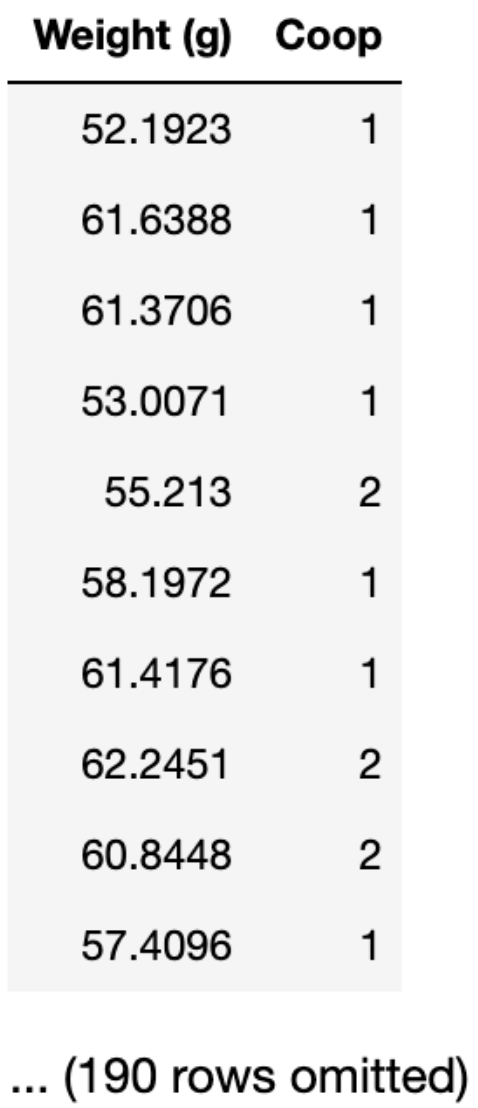
\includegraphics[scale=.35]{figures/chicken_table.png}
% \end{center}
% \begin{center}
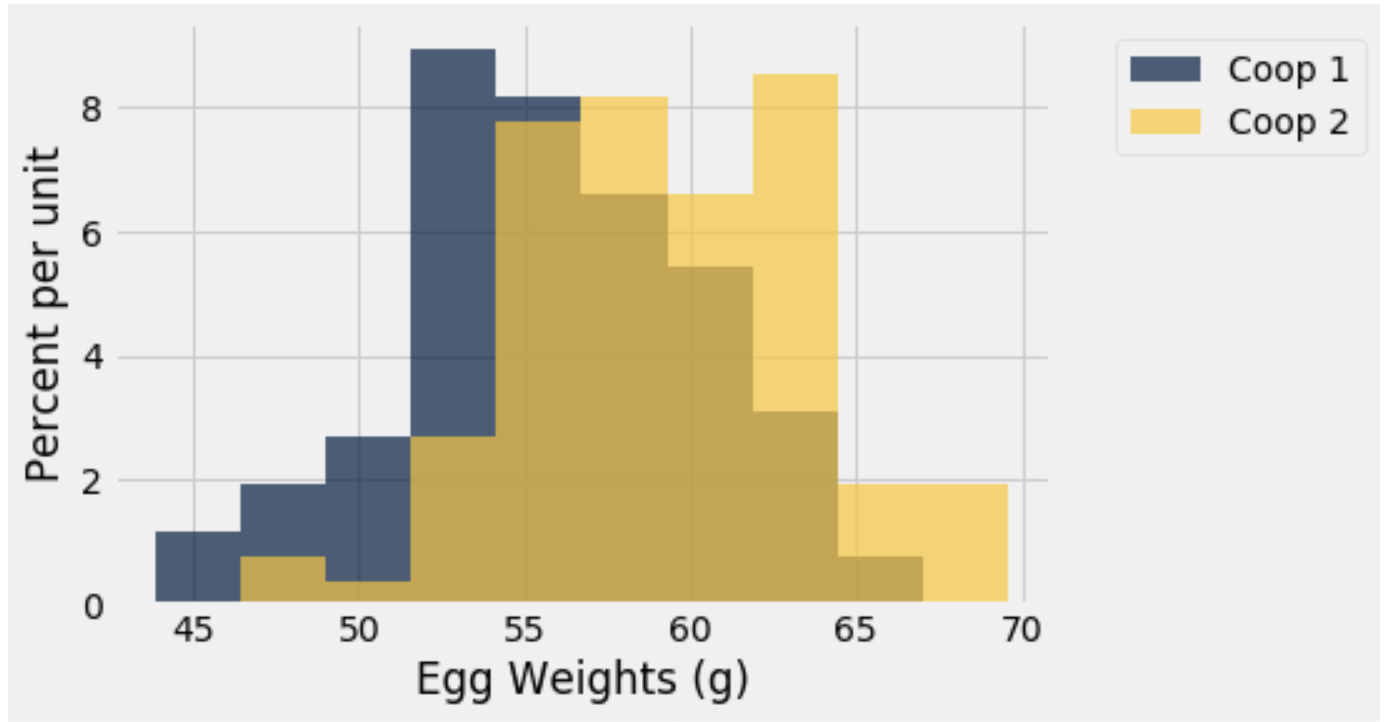
\includegraphics[scale=.55]{figures/chicken_hist.png}
% \end{center}
\vskip 0.2in
You want to conduct a hypothesis test to see if the distributions of egg weights come from one underlying distribution and thus support the idea that your chickens have no coop preference, or if instead the distributions of egg weights in the two coops are truly different. 

\vskip .05in
\begin{enumerate}

\subq{2} If we took a single bootstrapped resample of the Coop 1 eggs, what would the histogram of egg weights in our resampled table look like? 
\vskip 0.05in
\begin{enumerate}
    \bubble \quad The histogram would look like the Coop 1 histogram above, but narrower.\\[2pt]
    \bubble \quad The histogram would look like the Coop 1 histogram above,  but more normal.\\[2pt]
    \bubble \quad The histogram would be like the Coop 1 histogram above, but wider.\\[2pt]
    \solutionbubble \quad The histogram would not change very much from the Coop 1 histogram above. 
\end{enumerate}

\vskip .1in
\subq{2} How would you perform a single simulation under the null hypothesis that the distribution of weights in the two coops is the same?
\vskip 0.05in
\begin{enumerate}
    \bubble \quad Create two normal distributions centered at the mean of Coop 1 and Coop 2 and see if they overlap.\\[2pt]
    \solutionbubble \quad Shuffle the coop labels of your collected eggs and compute your test statistic on the shuffled table.\\[2pt]
    \bubble \quad Bootstrap the egg weights and calculate a new average egg weight.
\end{enumerate}

\vskip 1in    
\subq{2} What test statistic would \textbf{best} help differentiate between the null and the alternative hypothesis?
\vskip 0.05in
\begin{enumerate}
    \bubble \quad The Total Variation Distance (TVD) between the distribution of Coop 1 egg weights and Coop 2 egg weights. \\[2pt]
    \solutionbubble \quad The absolute value of the difference between the mean egg weight in Coop 1 and the mean egg weight in Coop 2.\\[2pt]
    \bubble \quad The mean egg weight of Coop 2.\\[2pt]
    \bubble \quad The difference between the mean egg weight in Coop  2 and Coop 1.
\end{enumerate}

\vskip .1in
\subq{4} Write a function \lsi+compute_one_test_stat+ that will take in the table with the same columns as \lsi+eggs+ above and returns one simulated value of your test statistic.
\vskip 0.05in
\solutionimage
{
{\lsi+def compute_one_test_stat(tbl):+}\\[10pt]
    \hspace*{0.5in}{\lsi+new_labels = +\bklong}\\[10pt]
    \hspace*{0.5in}{\lsi+new_table = +\bklong}\\[10pt]
    \hspace*{0.5in}{\lsi+means_col = +\bkshort+.+\bkshort+(+\bkshort+, +\bkshort+).+\bklong}\\[10pt]
    \hspace*{0.5in}{\lsi+test_stat = +\bklong}\\[10pt]
    \hspace*{0.5in}{\lsi+return test_stat+}
}
{
{\lsi+def compute_one_test_stat(tbl):+}\\[10pt]
    \hspace*{0.5in}{\lsi+new_labels = tbl.sample(with_replacement=False).column("Coop")+}\\[10pt]
    \hspace*{0.5in}{\lsi+new_table = tbl.with_columns("Shuffled labels", new_labels)+}\\[10pt]
    \hspace*{0.5in}{\lsi+means_col = new_table.group("Shuffled labels", np.mean).column('Weight (g) mean')+}\\[10pt]
    \hspace*{0.5in}{\lsi+test_stat = abs(means_col.item(0) - means_col.item(1))+}\\[10pt]
    \hspace*{0.5in}{\lsi+return test_stat+}
}
\vskip 0.1in
\subq{2} You use the \lsi+compute_one_test_stat+ function to compute the observed test statistic, which is stored in the variable \lsi+obsv_test_stat+, as well as 10,000 simulated test statistics,  which are stored in an array called \lsi+stats+.  Which of the following lines of code correctly computes the empirical p-value of this test? 
\vskip 0.05in
\begin{enumerate}
    \bubble \quad \lsi+np.count_nonzero(stats <= obsv_test_stat)/10000+\\[2pt]
    \solutionbubble \quad \lsi+np.count_nonzero(stats >= obsv_test_stat)/10000+\\[2pt]
    \bubble \quad \lsi+np.count_nonzero(stats == obsv_test_stat)/10000+\\[2pt]
    \bubble \quad \lsi+np.count_nonzero(stats >= 0.05)/100000+\\[2pt]
\end{enumerate}

\subq{4} \textbf{Select one of the options from parts i-ii to fill in the corresponding blanks in the sentence below.}

A larger observed difference in mean egg sizes would result in a \underline{\hspace{0.25in}}(i)\underline{\hspace{0.25in}} p-value. We would see a larger observed difference in mean egg sizes if Jersey Giant chickens exhibited a  \underline{\hspace{0.25in}}(ii)\underline{\hspace{0.25in}} preference for one coop, e.g. Coop 2.
\vskip 0.1in
\begin{enumerate}
    \item 
        {\solutionbubble} smaller\hspace{0.25in} {\bubble} larger
    \item
        {\bubble} weaker \hspace{0.25in}{\solutionbubble} stronger
\end{enumerate}

\vskip 0.1in
\subq{6} You calculate a p-value of 0.04 for this test. Select \textbf{all} true statements that we can justifiably conclude from this p-value. If you do not have enough information to evaluate whether the statement is true or false, DO NOT select it.
\vskip 0.05 in
\checkbox  There is a 4\% chance that the chickens have no preference for which coop they lay eggs in. \\
\checkbox  There is a 96\% chance that the chickens have no preference for which coop they lay eggs in.\\
\checkbox  If chickens actually have no coop preference, there is a 4\% chance we incorrectly reject the null hypothesis. \\
\solutionbox  We would reject the hypothesis that the chickens have no coop preference if we used a 5\% p-value cutoff.\\
\solutionbox   We would fail to reject the hypothesis that the chickens have no coop preference if we used a 1\% p-value cutoff.\\
\solutionbox   4\% of the simulated test statistics were greater than or equal to the observed test statistic.\\
\checkbox We cannot conclude any of the above options.

\end{enumerate}
